\section{Test Driven Development}
  Bevor wir in BDD eintauchen k"onnen m"ussen wir verstehen wie Test Driven 
  Development funktioniert, welche Vorteile es uns bringt und auf welche 
  Probleme wir sto"sen k"onnen.

  \subsection{Red-Green-Refactor}
    Grundlegend ist TDD ein Software Desing Process. Dieser Prozess basiert auf 
    der klaren Mantrik erst Tests f"ur einen nicht existenten Codeabschnitt zu
    schreiben, bevor der Code selbst implementiert wird.\\
    \begin{wrapfigure}{r}{0.5\textwidth}
      \vspace{-30pt}
      \begin{center}
        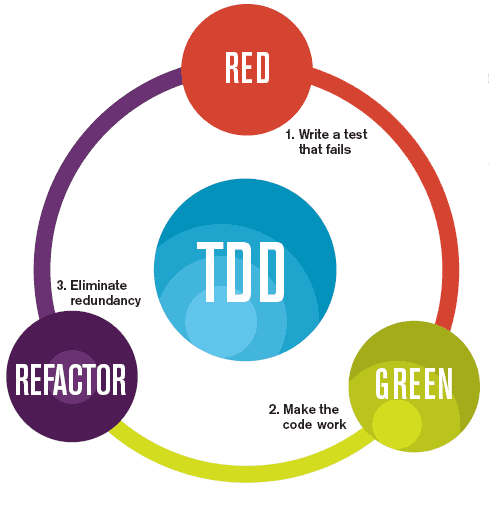
\includegraphics[scale=0.3]{assets/tdd_flow.png}
      \end{center}
      \caption{Red-Green-Refactor\cite{Osorio:2012}}
      \vspace{-15pt}
    \end{wrapfigure}
    Dies wird auch oft als 'Red-Green-Refactor-Zyklus' bezeichnet, da erst der Test
    ausgef"uhrt wird und fehlschl"agt, was bei den meisten Testingframeworks mit 
    Rot markiert wird, nun das Feature implementiert wird und der Test nicht 
    fehlschl"agt -dies wird oft mit Gr"un dargestellt.\\
    Sobald der Test nicht mehr feschl"agt betrachtet man das entstandene Design 
    des Features, reduziert Duplikate und kommentiert seinen Code. Nun kann man 
    ein weiteres mal in den Zyklus eintreten und die n"achsten Features wieder 
    nach dem gleichen System entwickeln.\\
    Ein Zyklus sollte allerdings nicht l"anger als 15 Minuten dauern. Falls doch
    hei"st dies entweder das zu implementierende Feature ist zu gro"s gew"ahlt
    oder der gew"ahlte L"osungsweg nicht optimal ist. Generell 
    sollten sich die Entwickler\_innen immer die Frage stellen ob Debuggen 
    schneller als neu implementieren eines Features ist, solange die Tests bei erst
    Implementierung fehlschlagen.

  \subsection{Auswirkungen und Vorteile}
    Sobald die Codebase w"achst wird immer mehr Zeit zum umstrukturieren des 
    bereits entwickelten Quellcodes ben"otigt und es wird sich langsam ein 
    sich konstant weiterentwickelndes Design herauskristallisieren.\\
    Durch diese evolvierende Art des Designs, auch 'Emergent Design'\cite[p.~4]{Chelimsky:2010} genannt, kann sich die Software und somit auch die 
    Entwickler\_innen dynamisch den Anforderungen des Stakeholders anpassen, was 
    besonders in agilen Softwareprozessen n"otig ist. Des weiteren ist es auf 
    Grund der 'Test First' Struktur stets m"oglich ein zumindest begrenzt 
    fertiges Produkt zu pr"asentieren, was sofortige Kommunikation und Feedback
    des Stakeholders erm"oglicht und schnell aufkommende Probleme in der Software
    sichtbar werden l"asst.\\

  \subsection{Bestehende und absehbare Probleme}
    Test Driven Development sollte nicht als Ersatz eines ausf"uhrlichen Testens
    der Software gesehen werden. Eher ist es als Prozess zusehen um qualitativen
    Quellcode an den der Entwicklung angeschlossenen Testzyklus zu "ubergeben.\\
    Doch genau das f"uhrt schnell zur Verwirrungen, da Entwickler\_innen dazu
    neigen TDD als M"oglichkeit zusehen sich diesen extra Testzyklus zu sparen.
    Dies f"uhrt dazu das w"ahrend des Entwickelns neuer Features nicht nur 
    Tests geschrieben werden die das Verhalten des Features nach au"sen spezifizieren
    sondern interne technische Details auf Funktion "uberpfr"ufen. Dadurch werden
    die Tests besonders von unerfahrenen TDD-Entwickler\_innen schnell zu 
    ausf"uhrlichem White-Box-Testing genutzt, was zu einer starken Verschr"ankung
    von Test-Suite und eigentlich Quellcode f"uhrt. Durch diese Verschr"ankung
    wird das im Zyklus enthaltene Umstrukturieren des Codes immer weiter 
    erschwert und die Test-Suite verliert an Wartbarkeit, da f"ur das von au"sen
    betrachtete Verhalten unwichtige technische Details bei "Anderungen zum 
    fehlschlagen der Tests f"uhren k"onnen.\\
    Speziell hierf"ur m"ussen die Entwickler\_innen Disziplin an den Tag legen,
    denn sie sind es die das "aussere Verhalten als Test implementieren und sich
    selbst davon abhalten m"ussen internes Verhalten zu testen.\\
    Ein strukturelles Problem bei TDD ist es, das die Entwickler\_innen selbst
    die Anforderungen der Stakeholder in Tests "ubersetzen m"ussen und es 
    dadurch dazu kommen kann das schon die Tests falsches verhalten pr"ufen
    und somit die Implementierung des Features gar nicht den Anforderungen 
    entsprechen kann. Au"serdem folgt aus der nicht klar gegebenen Nomenklatur
    f"ur Tests, dass sie zwar auf Grund ihrer Funktion das Verhalten der 
    Software dokumentieren, dies allerdings nur auf einer f"ur Entwickler\_innen
    lesbaren Ebene, obwohl nur der Stakeholder verifizieren k"onnnte, das die 
    Tests sein gew"unschtes Verhalten abdecken. Dies kann vielleicht durch 
    Erfahrung der Entwickler\_innen ausgeglichen werden indem sie klare 
    Methodennamen vergeben und durch viele Kommentare auch Menschen die nicht 
    im Programmieren bewandert sind die M"oglichkeit geben die Tests zu 
    verstehen.\\
    Allerdings muss nun jedes neue Teammitglied an diese speziellen Verfahren
    gew"ohnt werden, da sie auf Grund mangelnder Einheitlichkeit stark zwischen
    verschiedenen Teams varieren k"onnen.
    Ausserdem stellt sich f"ur die Entwickler immer die Frage bei welchem Feature
    sie nun mit Tests und Implementierung starten sollte, da sie ja nur die 
    "Ubersicht "uber alle Anforderungen des Stakeholders haben. Hierbei kann man
    als Richtlinie angeben das man von klein nach gro"s entwickeln sollte und 
    immer auf Funktionst"uchtigkeit des entstehenden Quellcodes achten sollte.\\
    Bei der Entwicklung eines Onlineshops f"angt man zum Beispiel als erstes 
    an Artikel einpflegen zu k"onnen, ohne Beachtung dessen das das nur f"ur
    Administratoren m"oglich sein sollte und erst sp"ater in der Entwicklung
    f"ugt man das Feature f"ur Logins hinzu.\\
    Es wird also eine inkrementelle Entwicklung gef"ordert, allerdings ben"otigt
    diese Erfahrung um sich nicht in Sackgassen in der Entwicklung zu verrennen.\\